\section{Training Neural Networks}
\begin{frame}{Training a Neural Network}
\begin{columns}[c]
    % ---------------- Left: text ----------------
    \begin{column}{0.30\textwidth}
        To train this model we repeat two phases:

        \vspace{2mm}
        \textbf{Forward Pass:}
        \begin{itemize}
            \item Data $\to$ Model $\to$ Predictions
            \item Compute Loss
        \end{itemize}

        \vspace{2mm}
        \textbf{Backward Pass:}
        \begin{itemize}
            \item Calculate gradients
            \item Update parameters
        \end{itemize}

        \vspace{2mm}
        \small \textit{Let’s discuss them in detail.}
    \end{column}

    % ---------------- Right: figure ----------------
    \begin{column}{0.70\textwidth}
        \centering
        \begin{tikzpicture}[
            scale=0.7,
            x=1.15cm, y=0.75cm,
            >={Latex[length=2.2mm]},
            neuron/.style={circle, draw=black, fill=white, line width=0.6pt, minimum size=4.6mm, inner sep=0pt},
            conn/.style={draw=black!55, line width=0.45pt},
            lab/.style={font=\scriptsize}
        ]
        % ---- Layer x positions ----
        \def\xIn{0}
        \def\xHone{2.0}
        \def\xHtwo{3.6}
        \def\xDots{5.0}
        \def\xHn{6.4}
        \def\xOut{8.0}

        % ---- Nodes ----
        % Input layer (6)
        \foreach \i/\yy in {1/2.5,2/1.5,3/0.5,4/-0.5,5/-1.5,6/-2.5}{
            \node[neuron] (I\i) at (\xIn,\yy) {};
        }

        % Hidden layer 1 (3 shown + dots)
        \foreach \i/\yy in {1/2.0,2/1.0,3/0.0}{
            \node[neuron] (Hone\i) at (\xHone,\yy) {};
        }
        \node[lab] at (\xHone,-1.0) {$\vdots$};
        \node[neuron] (Hone4) at (\xHone,-2.0) {};

        % Hidden layer 2 (2 shown + dots)
        \foreach \i/\yy in {1/1.7,2/0.7}{
            \node[neuron] (Htwo\i) at (\xHtwo,\yy) {};
        }
        \node[lab] at (\xHtwo,-0.3) {$\vdots$};
        \node[neuron] (Htwo3) at (\xHtwo,-1.7) {};

        % Middle dots column (just to indicate more layers)
        \foreach \k/\yy in {1/1.7,2/0.7,3/-0.3,4/-1.3}{
            \node[lab] at (\xDots,\yy) {$\cdot$};
        }

        % Hidden layer n (3 shown + dots)
        \foreach \i/\yy in {1/1.7,2/0.7,3/-1.7}{
            \node[neuron] (Hn\i) at (\xHn,\yy) {};
        }
        \node[lab] at (\xHn,-0.5) {$\vdots$};

        % Output (single)
        \node[neuron] (O) at (\xOut,0.0) {};

        % ---- Connections (dense-ish but readable) ----
        \foreach \i in {1,...,6}{
            \foreach \j in {1,2,3,4}{
                \draw[conn] (I\i) -- (Hone\j);
            }
        }
        \foreach \j in {1,2,3,4}{
            \foreach \k in {1,2,3}{
                \draw[conn] (Hone\j) -- (Htwo\k);
            }
        }
        % connect H2 -> Hn (skip dots, just imply)
        \foreach \k in {1,2,3}{
            \foreach \m in {1,2,3}{
                \draw[conn] (Htwo\k) -- (Hn\m);
            }
        }
        \foreach \m in {1,2,3}{
            \draw[conn] (Hn\m) -- (O);
        }

        % ---- Labels ----
        \node[lab, align=center] at (\xIn,3.55) {Input\\layer};
        \node[lab, align=center] at (\xHone,-3.05) {Hidden\\layer 1};
        \node[lab, align=center] at (\xHtwo,-3.05) {Hidden\\layer 2};
        \node[lab, align=center] at (\xHn,-3.05) {Hidden\\layer $n$};
        \node[lab, align=center] at (\xOut,1.0) {Output\\layer};

        % ---- Forward / backward arrows ----
        \draw[->, line width=0.9pt] (\xIn0.4,3.6) -- (\xOut+0.2,3.6);
        \node[lab] at ($( \xIn-0.2,4.0)!0.45!(\xOut+0.2,4.0) $) {Forward pass};

        \draw[->, line width=0.9pt] (\xOut+0.2,-3.75) -- (\xIn-0.2,-3.75);
        \node[lab] at ($( \xOut+0.2,-4.25)!0.55!(\xIn-0.2,-4.25) $) {Backward pass};

        \end{tikzpicture}
    \end{column}
\end{columns}
\end{frame}



\section{Training a Neural Network}

\begin{frame}{1. Forward Pass}
\textbf{Goal:} Compute the network output $\hat{y}$ from input $x$, then measure the error.

\vspace{0.8em}
\begin{columns}[c]
\begin{column}{0.50\textwidth}
\textbf{What happens (layer by layer):}
\begin{enumerate}
    \item Start with input: $a^{(0)} = x$.
    \item For each layer $\ell$:
    \[
        z^{(\ell)} = W^{(\ell)} a^{(\ell-1)} + b^{(\ell)}   
    \]
    \[
        a^{(\ell)} = \sigma\!\left(z^{(\ell)}\right)
    \]
    \item Final layer gives the prediction: $\hat{y} = a^{(L)}$.
    \item \textbf{Loss:} $J(\theta)$ compares $\hat{y}$ with the true target $y$.
\end{enumerate}

\vspace{0.3em}
\small \textit{Forward pass = just prediction (no learning yet).}
\end{column}

\begin{column}{0.50\textwidth}

\centering
\begin{tikzpicture}[scale=0.8, node distance=1.5cm, auto, thick]
\node[circle, draw, fill=green!20] (x) {$x$};
\node[circle, draw, fill=blue!20, right=of x] (h) {$h$};
\node[circle, draw, fill=red!20, right=of h] (y) {$\hat{y}$};

\draw[->] (x) -- node[above, font=\scriptsize] {$W^{(1)},b^{(1)}$} (h);
\draw[->] (h) -- node[above, font=\scriptsize] {$W^{(2)},b^{(2)}$} (y);

\node[below=0.5cm of y, red] (loss) {Loss $J(\hat{y},y)$};
\draw[dashed, ->] (y) -- (loss);
\end{tikzpicture}
\end{column}
\end{columns}
\end{frame}


% =========================
% Backpropagation = Chain Rule (clean + example)
% =========================

% --- SLIDE: What is Backprop ---
\begin{frame}{2. Backward Pass (Backpropagation)}
    \textbf{Goal:} Given feedback from the loss, calculate gradients for all weights, then update them via Gradient Descent.
    
    \vspace{0.8em}
    By applying the \textbf{Chain Rule}, we multiply these partial derivatives to derive the gradient for every parameter. 
    
    We move from the end (the loss) \textbf{backwards} towards the beginning, passing through each weight to get its gradient. This is called \textbf{Backpropagation}.
    
    % \vspace{0.8em}
    \centering
    \begin{tikzpicture}[node distance=1.7cm, thick, scale=0.4]
        % nodes
        \node[draw, circle, fill=green!15, minimum size=0.9cm] (x) {$x$};
        \node[draw, rectangle, rounded corners, fill=blue!10, minimum height=0.9cm, minimum width=1.6cm, right=of x] (z) {$z=wx+b$};
        \node[draw, rectangle, rounded corners, fill=blue!10, minimum height=0.9cm, minimum width=1.6cm, right=of z] (a) {$a=\sigma(z)$};
        \node[draw, rectangle, rounded corners, fill=red!10, minimum height=0.9cm, minimum width=1.6cm, right=of a] (J) {$J(a,y)$};
        
        % arrows
        \draw[->] (x) -- (z);
        \draw[->] (z) -- (a);
        \draw[->] (a) -- (J);
        
        % y
        \node[draw, circle, fill=red!10, minimum size=0.9cm, below=0.9cm of J] (y) {$y$};
        \draw[->] (y) -- (J);
        
        % local derivatives
        \node[above=0.10cm of J, font=\small]  {$\frac{\partial J}{\partial a}$};
        \node[above=0.10cm of a, font=\small]  {$\frac{\partial a}{\partial z}$};
        \node[above=0.10cm of z, font=\small]  {$\frac{\partial z}{\partial w}$};
    \end{tikzpicture}
    
    % \vspace{0.5em}
    % \small Backpropagation = Multiplying these **derivatives** along the path to get the gradient for each parameter.
\end{frame}


% --- SLIDE: Chain Rule example (symbolic, super clear) ---
\begin{frame}{Chain Rule Example: Compute $\frac{\partial J}{\partial w}$}
Assume one neuron:
\[
z=wx+b,\quad a=\sigma(z),\quad J=\frac{1}{2}(a-y)^2
\]

\begin{tcolorbox}[colback=yellow!8, colframe=orange!70, title=\textbf{Chain Rule (backprop)}]
\[
\frac{\partial J}{\partial w}
=
\frac{\partial J}{\partial a}
\cdot
\frac{\partial a}{\partial z}
\cdot
\frac{\partial z}{\partial w}
\]
\end{tcolorbox}

\vspace{0.5em}
Now compute each piece:
\[
\frac{\partial J}{\partial a} = (a-y)
\qquad
\frac{\partial a}{\partial z} = \sigma(z)(1-\sigma(z)) = a(1-a)
\qquad
\frac{\partial z}{\partial w} = x
\]

\begin{block}{Final result}
\[
\boxed{
\frac{\partial J}{\partial w} = (a-y)\,a(1-a)\,x
}
\]
\end{block}
\end{frame}

% --- SLIDE: Using the gradient to update parameters (no optimizer details) ---
\begin{frame}{Using the Gradient to Update Parameters}
\textbf{What do we do with } $\frac{\partial J}{\partial w}$ \textbf{?}  
We use Gradient Descent to update the weights.

\vspace{0.8em}
\begin{tcolorbox}[colback=green!6, colframe=green!50!black, title=\textbf{Parameter Update Rule (via Gradient Descent)}]
\[
w \leftarrow w - \alpha \,\frac{\partial J}{\partial w}
\qquad
b \leftarrow b - \alpha \,\frac{\partial J}{\partial b}
\]
\end{tcolorbox}

\vspace{0.6em}
\small
\begin{itemize}
    \item $\alpha$ : learning rate (step size).
    \item We compute $\frac{\partial J}{\partial(\cdot)}$ for \textbf{every} parameter using backprop.
\end{itemize}

\pause
\begin{tcolorbox}[colback=yellow!8, colframe=orange!70, arc=8pt]
\centering
\textbf{Q:}
Do we do this update using \textbf{all data at once}?
\end{tcolorbox}
\end{frame}





% \begin{frame}{4. The Update (Optimization)}
% \textbf{Gradient} points in the direction that \textbf{increases} the loss.
% So we move in the opposite direction to reduce it.

% \vspace{0.8em}
% \begin{tcolorbox}[colback=green!5, colframe=green!50!black, title=\textbf{Gradient Descent Update}]
% \[
% \theta \leftarrow \theta - \alpha \,\nabla_\theta J(\theta)
% \]
% \end{tcolorbox}

% \vspace{0.8em}
% \begin{itemize}
% \item $\theta$: all parameters (weights and biases).
% \item $\alpha$: learning rate (step size).
% \item $\nabla_\theta J$: gradients computed by backprop.
% \end{itemize}

% \vspace{0.4em}
% \small \textit{Repeat: forward $\rightarrow$ loss $\rightarrow$ backward $\rightarrow$ update.}
% \end{frame}




% --- SLIDE 17: Step (One Update) ---
\begin{frame}{Training Step = One Update}
\textbf{We do not train using the full dataset at once.}
\vspace{0.7em}

Instead, we take a \textbf{small batch} (mini-dataset) and do one update:

\vspace{0.8em}
\centering
\begin{tikzpicture}[
    font=\small,
    >={Latex[length=2mm]},
    box/.style={draw, rounded corners, thick, minimum height=7mm},
    data/.style={box, fill=gray!10, minimum width=8.0cm},
    batch/.style={box, fill=blue!10, minimum width=1.55cm},
    batchHi/.style={box, fill=blue!25, minimum width=1.75cm},
    flow/.style={box, fill=blue!5, minimum width=8.0cm}
]
% Dataset
\node[data] (D) {Full Training Dataset};
% Batches row (one highlighted)
\node[batch]   (b1) at (-3.0,-1.1) {Batch 1};
\node[batch]   (b2) at (-1.2,-1.1) {Batch 2};
\node[font=\tiny] (dots) at (-0.23,-1.1) {$\cdots$};
\node[batchHi] (b3) at (0.8,-1.1) {\textbf{Batch $k$}};
\node[batch]   (b4) at (2.8,-1.1) {Batch $k\!+\!1$};
% arrows down - now pointing to EACH batch
\draw[->, black!55] (D.south) -- (b1.north);
\draw[->, black!55] (D.south) -- (b2.north);
\draw[->, black!55] (D.south) -- (b3.north);
\draw[->, black!55] (D.south) -- (b4.north);
% flow box
\node[flow, align=center] (F) at (0,-2.3)
{\textbf{Forward} $\rightarrow$ \textbf{Loss} $\rightarrow$ \textbf{Backward} $\rightarrow$ \textbf{Update}};
\draw[->, black!55] (b3.south) -- (F.north);
\end{tikzpicture}
\vspace{0.7em}
\begin{itemize}
\item This single update is called a \textbf{training step} (or \textbf{iteration}).
\item \textbf{Batch size} = how many samples are used in one step.
\end{itemize}
\vspace{0.4em}
\small \textit{Next: repeat this step for \textbf{all} batches $\Rightarrow$ one full \textbf{epoch}.}
\end{frame}

% --- SLIDE 18: Epoch (Full Pass) ---
\begin{frame}{Epoch = One Full Pass Over the Dataset}
\textbf{Dataset} $\rightarrow$ split into \textbf{batches} $\rightarrow$ each batch makes \textbf{one step}.

\vspace{0.9em}
\centering
\begin{tikzpicture}[
    font=\small,
    >={Latex[length=2mm]},
    box/.style={draw, rounded corners, thick, minimum height=7mm},
    data/.style={box, fill=gray!10, minimum width=8.0cm},
    batch/.style={box, fill=blue!10, minimum width=1.55cm},
]
% Dataset
\node[data] (D) {Full Training Dataset};
% Batches row
\node[batch] (b1) at (-3.0,-1.1) {Batch 1};
\node[batch] (b2) at (-1.2,-1.1) {Batch 2};
\node[font=\tiny] (dots) at (-0.23,-1.1) {$\cdots$};
\node[batch] (b3) at (0.8,-1.1) {Batch $k$};
\node[batch] (b4) at (2.8,-1.1) {Batch $N$};
% arrows down - pointing to each batch
\draw[->, black!55] (D.south) -- (b1.north);
\draw[->, black!55] (D.south) -- (b2.north);
\draw[->, black!55] (D.south) -- (b3.north);
\draw[->, black!55] (D.south) -- (b4.north);
% bracket = epoch (opening upward)
\draw[decorate, decoration={brace, amplitude=6pt, mirror}, thick]
(-3.7,-1.75) -- (3.5,-1.75);
\node[font=\small] at (0,-2.25) {\textbf{1 Epoch} = all batches processed once};
\end{tikzpicture}
% \vspace{0.8em}
\begin{itemize}
\item \textbf{Steps per epoch} $\approx \left\lceil \frac{\#\text{samples}}{\text{batch size}} \right\rceil$.
\item Training usually runs for \textbf{many epochs}.
\end{itemize}
\vspace{0.3em}
\small \textit{Next: before the next epoch, we usually \textbf{shuffle} the dataset.}
\end{frame}
% --- SLIDE 19: Shuffling (Why it helps) ---
\begin{frame}{Why Shuffle Between Epochs?}
\textbf{At the start of each epoch, we shuffle the dataset to randomize batch composition.}
\vspace{1em}

\begin{columns}[T]
\begin{column}{0.48\textwidth}
\textbf{Without shuffling:}
\begin{itemize}
\item Batches see same patterns repeatedly
\item Similar samples grouped together
\item Biased gradient estimates
\end{itemize}
\vspace{0.5em}
\textbf{With shuffling:}
\begin{itemize}
\item Each batch is a better mix
\item More stable learning
\item Better generalization
\end{itemize}
\end{column}

\begin{column}{0.48\textwidth}
\centering
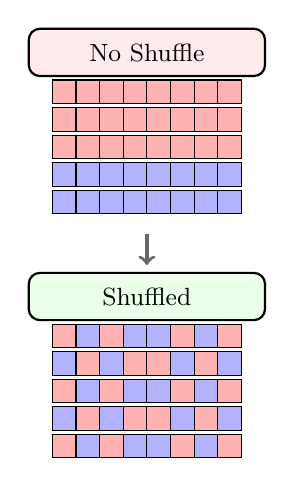
\begin{tikzpicture}[
    box/.style={draw, rounded corners, thick, minimum width=3cm, minimum height=0.6cm, font=\small},
    cell/.style={draw, minimum width=3mm, minimum height=3mm},
]
% No shuffle
\node[box, fill=red!8] (ns) at (0,0) {No Shuffle};
\foreach \r in {0,1,2} {
  \foreach \c in {0,...,7} {
    \node[cell, fill=red!30] at (-1.05+\c*0.3, -0.5-\r*0.35) {};
  }
}
\foreach \r in {0,1} {
  \foreach \c in {0,...,7} {
    \node[cell, fill=blue!30] at (-1.05+\c*0.3, -1.55-\r*0.35) {};
  }
}

% Arrow
\draw[->, very thick, black!60] (0,-2.3) -- (0,-2.7);

% Shuffled (5 rows)
\node[box, fill=green!8] (s) at (0,-3.1) {Shuffled};
\foreach \i/\c/\col in {
  0/0/red!30, 1/1/blue!30, 2/2/red!30, 3/3/blue!30,
  4/4/blue!30, 5/5/red!30, 6/6/blue!30, 7/7/red!30,
  8/0/blue!30, 9/1/red!30, 10/2/blue!30, 11/3/red!30,
  12/4/red!30, 13/5/blue!30, 14/6/red!30, 15/7/blue!30,
  16/0/red!30, 17/1/blue!30, 18/2/red!30, 19/3/blue!30,
  20/4/blue!30, 21/5/red!30, 22/6/blue!30, 23/7/red!30,
  24/0/blue!30, 25/1/red!30, 26/2/blue!30, 27/3/red!30,
  28/4/red!30, 29/5/blue!30, 30/6/red!30, 31/7/blue!30,
  32/0/red!30, 33/1/blue!30, 34/2/red!30, 35/3/blue!30,
  36/4/blue!30, 37/5/red!30, 38/6/blue!30, 39/7/red!30
}{
  \pgfmathtruncatemacro{\row}{int(\i/8)}
  \node[cell, fill=\col] at (-1.05+\c*0.3, -3.6-\row*0.35) {};
}
\end{tikzpicture}
\end{column}
\end{columns}
\end{frame}


\section{A Deep Dive into Optimizers}

% --- TRANSITION: THE THREE PILLARS (Optim Highlighted) ---
